\parindent=0em
\subsection{HP VR1000-127il}
\noindent

Este HMD de la empresa HP salió al mercado en el año 2018, es un dispositivo dependiente de un ordenador compatible con la plataforma \textit{Windows Mixed Reality}. Este casco se conecta a dicho ordenador a través de una conexión 2 en 1 que combina un HMDI 2.0 y USB 3.0. \\

Las gafas \textit{HP VR1000-123il} (figura~\ref{fig:hpvr1000}) utilizan dos controladores inalámbricos (que se conectan mediante \textit{bluetooth}) para controlar el movimiento de las manos, estos controladores utilizan 2 pilas AA cada uno. El dispositivo tiene un campo de visión de 90\degree  y una resolución de 1.440×1.440 píxeles por ojo (un total de 2.880x1.440 píxeles con ambos ojos), por otro lado, el casco cuenta con 6DoF y la IPD no se puede regular. 

\begin{figure}[H]
    \centering
    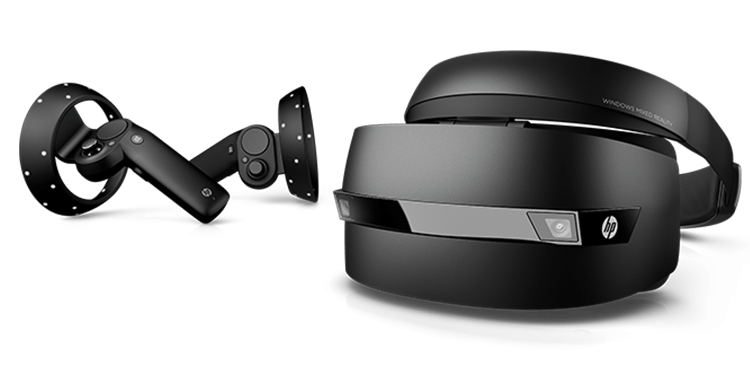
\includegraphics[scale=0.5]{Images/Estado del arte/HP VR1000.png}
    \caption[\textit{HP VR1000-123il} y sus controladores]{\textit{HP VR1000-123il} y sus controladores\footnotemark.}
    \label{fig:hpvr1000}
\end{figure}

\footnotetext{Fuente: \href{https://store.hp.com/SpainStore/Merch/Offer.aspx?p=c-auriculares-realidad-mixta&utm_source=affiliate&utm_medium=cpa&utm_campaign=Compradicci\%c3\%b3n&utm_content=21683024&jumpid=af_vr4n6qubez/site:Compradicci\%c3\%b3n}{\nolinkurl{https://store.hp.com/HP VR1000-123il}}}
Finalmente, este HMD no tiene un diseño centrado en su uso con gafas y tiene un peso de 834 gramos. 